
\documentclass[preprint,12pt]{elsarticle}

\usepackage[spanish]{babel}
\usepackage{amssymb}
\usepackage{graphicx}
\usepackage{lineno}
\usepackage[utf8]{inputenc}
\usepackage{url}
\usepackage{natbib}
\usepackage{float}
\begin{document}
	


	\begin{frontmatter}

		\title{\huge  DevOps En Base de Datos}
		
		\author{José Edilberto Pastor Mendoza              (2016055237)}
		\author{MAMANI MAMANI, Pedro Luis              (2010038808)}
		\author{PACORA SILVA, Jorge Carlos                   (2013000725)}
		\author{PANTY SIHUAYRO, Juan Carlos               (2014049452)}
		
		\address{Tacna, Perú}
		
		\begin{abstract}
			
Building great software is not just about code. It is also on the management of multiple teams, schedules and frequently Changes, DevOps has become an effective way to help teams collaborate and accelerate the delivery cycle. One of the biggest advantages is development automation and repetitive testing. processes used by database development teams to deliver, manage and maintain the database. From the version that controls changes to deployment in different environments, and when ready, choose to deploy in production, continuous delivery helps teams reduce risk and increase both efficiency and reliability in the software launch process.


		\end{abstract}
\end{frontmatter}

	\section{Resumen}

Construir un gran software no solamente se trata del código. Es también 
sobre la gestión de múltiples equipos, plazos y con frecuencia
Cambios , DevOps se ha convertido en una forma efectiva de ayudar a los equipos a colaborar y acelerar el ciclo de entrega.
Una de las mayores ventajas es la automatización del desarrollo y las pruebas repetitivas.
procesos que utilizan los equipos de desarrollo de bases de datos para entregar, administrar y mantener la base de datos. Desde la versión que controla los cambios hasta la implementación en diferentes entornos, y cuando esté listo, elegir desplegarse en producción, la entrega continua ayuda a los equipos a reducir
arriesgar e incrementar tanto la eficiencia como la confiabilidad en el proceso de lanzamiento del software.


\section{Introduccion}
En DevOps para entornos de prueba de bases de datos, las organizaciones deben generar rápidamente clones del sistema para ofrecer datos que reflejen con precisión el entorno de producción, al tiempo que protegen la información corporativa sensible. Por otro lado, los cambios de la base de datos en la producción representan el abismo más amplio entre las técnicas de desarrollo de aplicaciones ágil y la capacidad de desplegarlas en infraestructuras de TI del mundo real.
CI / CD no es un concepto nuevo y es realmente el punto central de cada implementación de DevOps. He allí que en este articulo nos ocupamos del modo puntual sobre los conceptos basicos de devops, como se desenvuelve en un entorno de base de datos y que herramientas pueden usarse.
	
	
\section{Marco Teorico}
	
\subsection{DEFINICIONES DE DEVOPS}	

Según (Bass, L., Weber, I., Zhu, L., (2015), DevOps A Software Architect’s Perspective, (Edi.) Addison-Wesley Professional, Boston) “DevOps es un conjunto de prácticas destinadas a reducir el tiempo entre el compromiso de un cambio en un sistema y el cambio que se coloca en la producción normal, al tiempo que garantiza una alta calidad.”.

Según (Huttermann, M., (2012), Devops for Developers, (Edi.) Apress, España)” DevOps es una mezcla de patrones destinados a mejorar la colaboración entre desarrollo y operaciones. Direcciones DevOps compartidas Objetivos e incentivos, así como procesos y herramientas compartidos. Porque de los conflictos naturales entre los diferentes grupos, objetivos compartidos y Los incentivos no siempre son alcanzables. Sin embargo, deberían en menos estar alineados unos con otros.”.
\begin{figure}[H]
				\begin{center}
					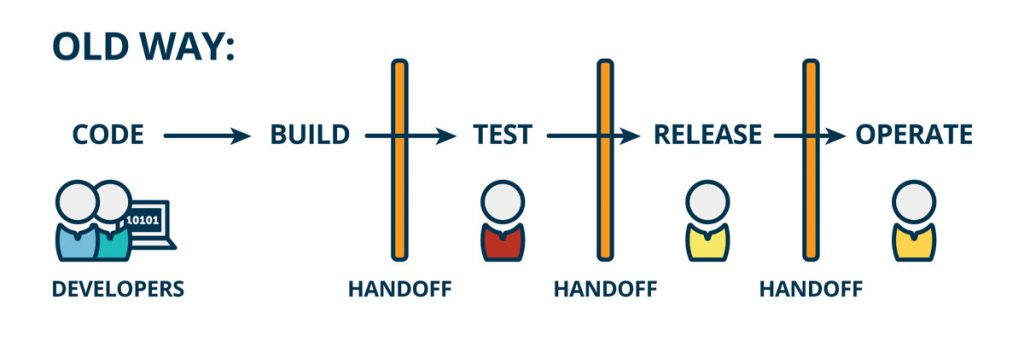
\includegraphics[width=12cm,height=7cm]{./IMAGENES/devops1}
				\end{center}
Maheta,H.(2018).What is DevOps and Why DevOps:.[Figura].Recuperado de 
https://www.yudiz.com/welcome-devops-prevent-defects/

			\end{figure}



\subsection{¿Qué es la integración continua/distribución continua (CI/CD)?}	
La CI/CD es un método para distribuir aplicaciones de forma frecuente a los clientes mediante el uso de la automatización en las etapas del desarrollo de las aplicaciones. Los principales conceptos que se atribuyen a la CI/CD son la integración continua, la distribución continua y la implementación continua.(Redhat, 2019) 
\begin{itemize}
\item Integración continua 
\item Distribución continua
\end{itemize}
	\begin{figure}[H]
			\begin{center}
					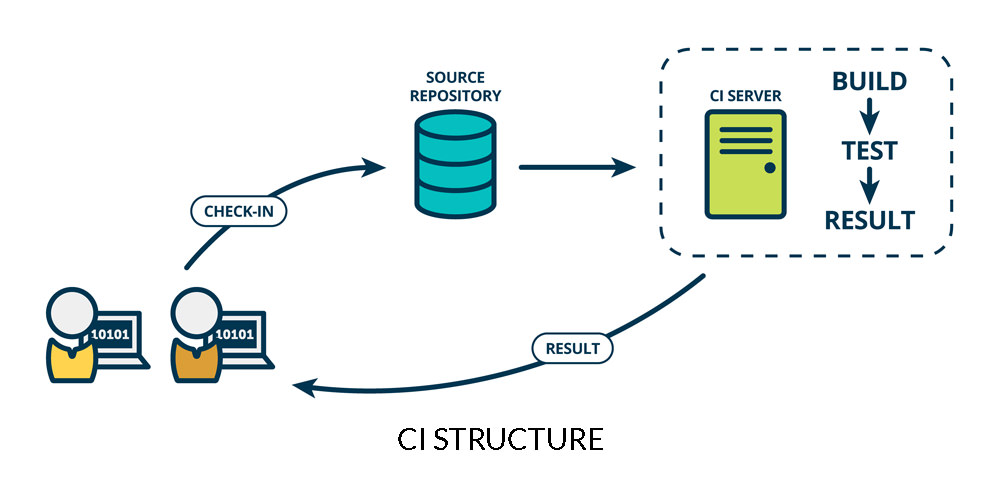
\includegraphics[width=12cm,height=7cm]{./IMAGENES/devops2}
					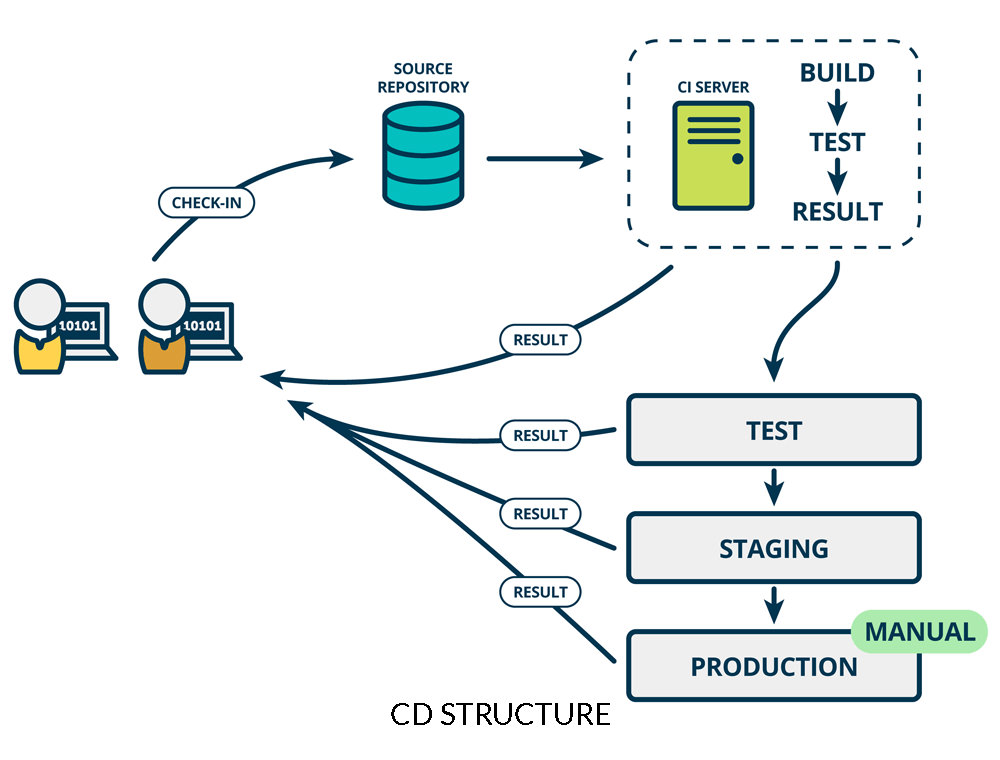
\includegraphics[width=12cm,height=7cm]{./IMAGENES/devops3}
			\end{center}
			Maheta,H.(2018).What is DevOps and Why DevOps:.[Figura].Recuperado de 
https://www.yudiz.com/welcome-devops-prevent-defects/
		\end{figure}



\subsection{DevOps para bases de datos}	


Adoptar una cultura DevOps le permite implementar códigos más rápido, lo que significa que puede crear, probar y lanzar cambios de software más rápido. Esto, a su vez, lleva a un 21 \% de reducción del trabajo no planificado y de las reelaboraciones y un 19 \% de aumento en los ingresos*. Cuando usted alinee cambios en bases de datos y aplicaciones en un flujo de trabajo integrado, ejecutará funciones de administración de cambios en bases de datos fundamentales dentro de su flujo de trabajo de DevOps sin comprometer la calidad, el rendimiento ni la confiabilidad.\citep{referencia10}


\subsection{La nube para DevOps}

La nube está posicionada de manera única para funcionar como la infraestructura para un abordaje de DevOps por muchas razones, que incluyen:
\begin{itemize}

\item La nube se define por software; es programable y flexible.
\item La nube se acciona por software y tiene muchas capas. El cliente es responsable por cada capa y debe diseñarla, desde la configuración para la cuenta de servicios y credenciales hasta la protección de los datos y los valores de cifrado.\citep{referencia09}
\end{itemize} 


\section{Analisis}

La solución técnica para aplicar DevOps a la base de datos es agregar o generar scripts SQL en la canalización de CI y desplegarlos durante el CD.
Tenemos 2 opciones principales: una con migraciones ORM y otra con proyecto de base de datos. Construiremos la muestra usando SQL Server, ASP.NET Core, EF Core y Azure DevOps. Pero, el mismo concepto podría aplicarse a otras tecnologías similares.

\subsection{Los ORM pueden permitir migraciones de bases de datos de forma transparente}
Los ORM como Entity Framework (EF), Doctrine, Hibernate (con Liquibase o Flyway) tienen funciones integradas para migraciones automáticas de código primero. Pueden detectar cambios en las entidades del objeto, generar el script SQL correspondiente e implementarlo en la base de datos.
Las migraciones automáticas podrían habilitarse en EF mediante el comando cli ' dotnet ef migrations add AddedColor ' y agregar el siguiente código: Context.Database.Migrate ();.

EF creará una carpeta de Migraciones dentro del código fuente de nuestra aplicación. Luego creará objetos de migración que contienen el nuevo cambio a través del método Up escrito con los objetos ORM. Observe en la siguiente imagen, el método AddColumn que se traducirá más tarde, por EF, durante la implementación, en una operación SQL ALTER TABLE.

	\begin{figure}[H]
			\begin{center}
					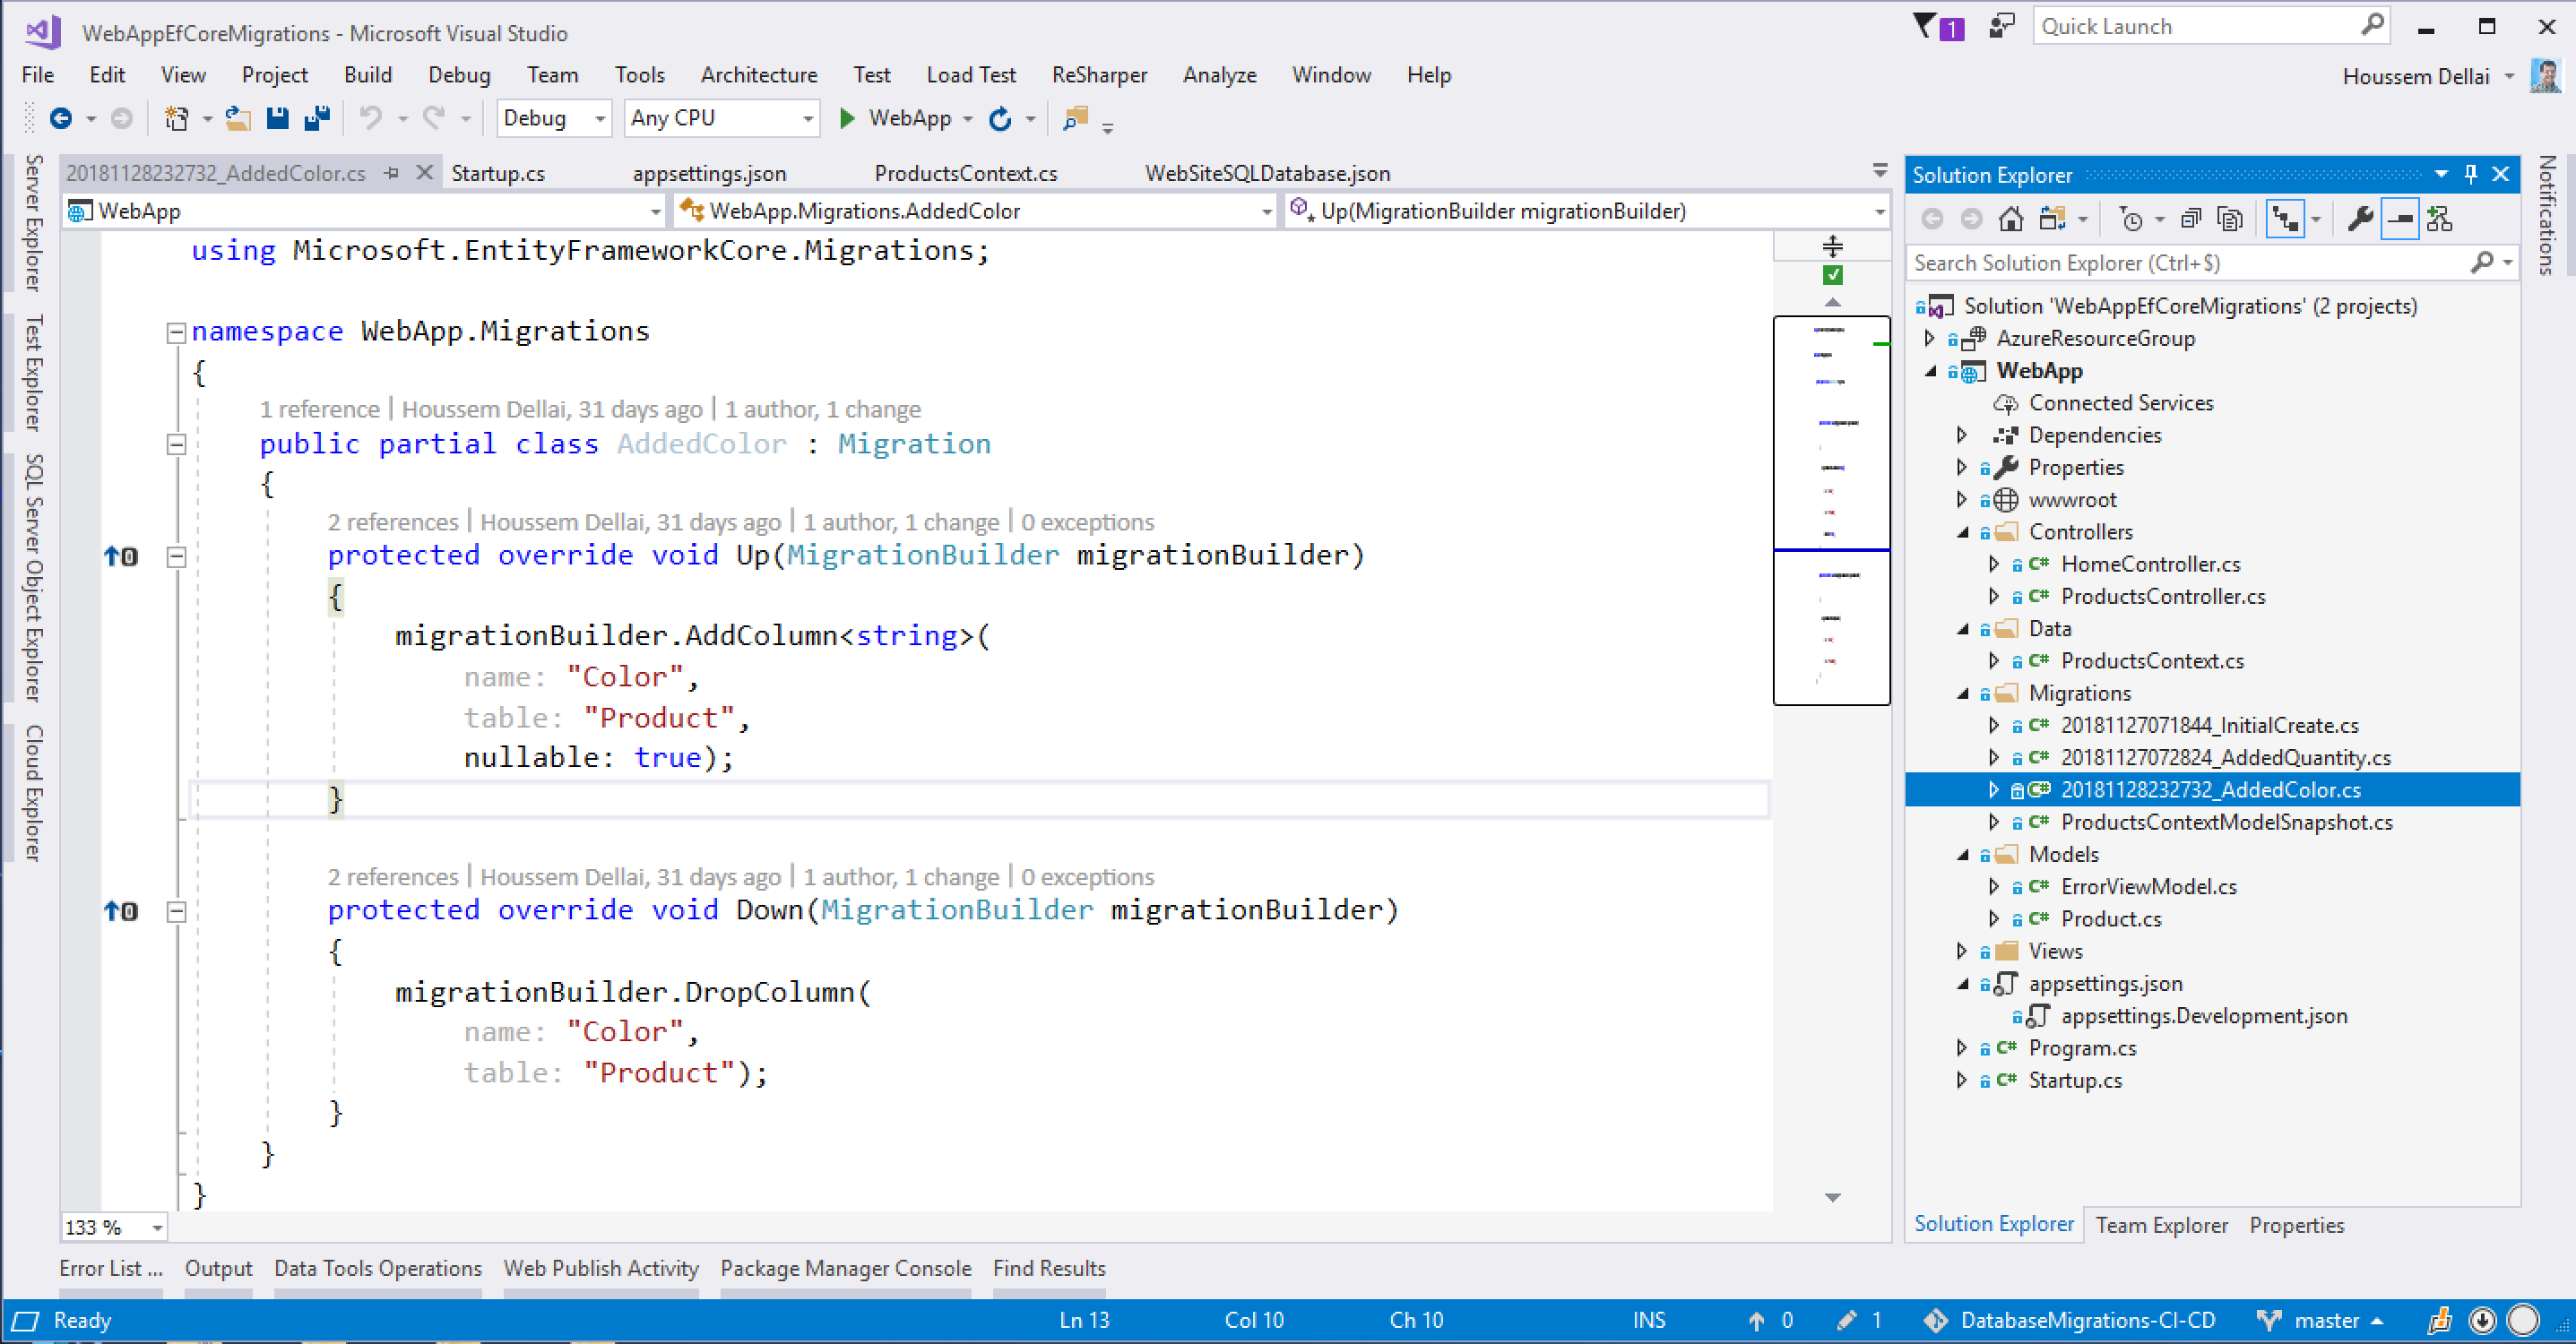
\includegraphics[width=12cm,height=7cm]{./IMAGENES/analisis1}
			\end{center}
			Houssem Dellai(2018).DevOps para la base de datos:.[Figura].Recuperado de 
https://medium.com/faun/devops-for-database-4e442abfd939
		\end{figure}

Tenga en cuenta también, el uso del método Down que se utiliza para revertir los cambios realizados por el método Up. Eso es útil para los escenarios de Rollback.
Con eso en su lugar, no necesita cambiar nada en sus canalizaciones de CI / CD. El ORM generará e implementará los scripts SQL de migración de forma transparente. Nuestra canalización de Build / CI tendrá el siguiente aspecto en Azure DevOps: todas las tareas son para restaurar, compilar, probar unidades y publicar el código fuente de la aplicación, nada especial para la base de datos. Tenga en cuenta la última tarea utilizada para publicar la plantilla ARM creada por Ops para crear la infraestructura necesaria para ejecutar la aplicación en Azure.

	\begin{figure}[H]
			\begin{center}
					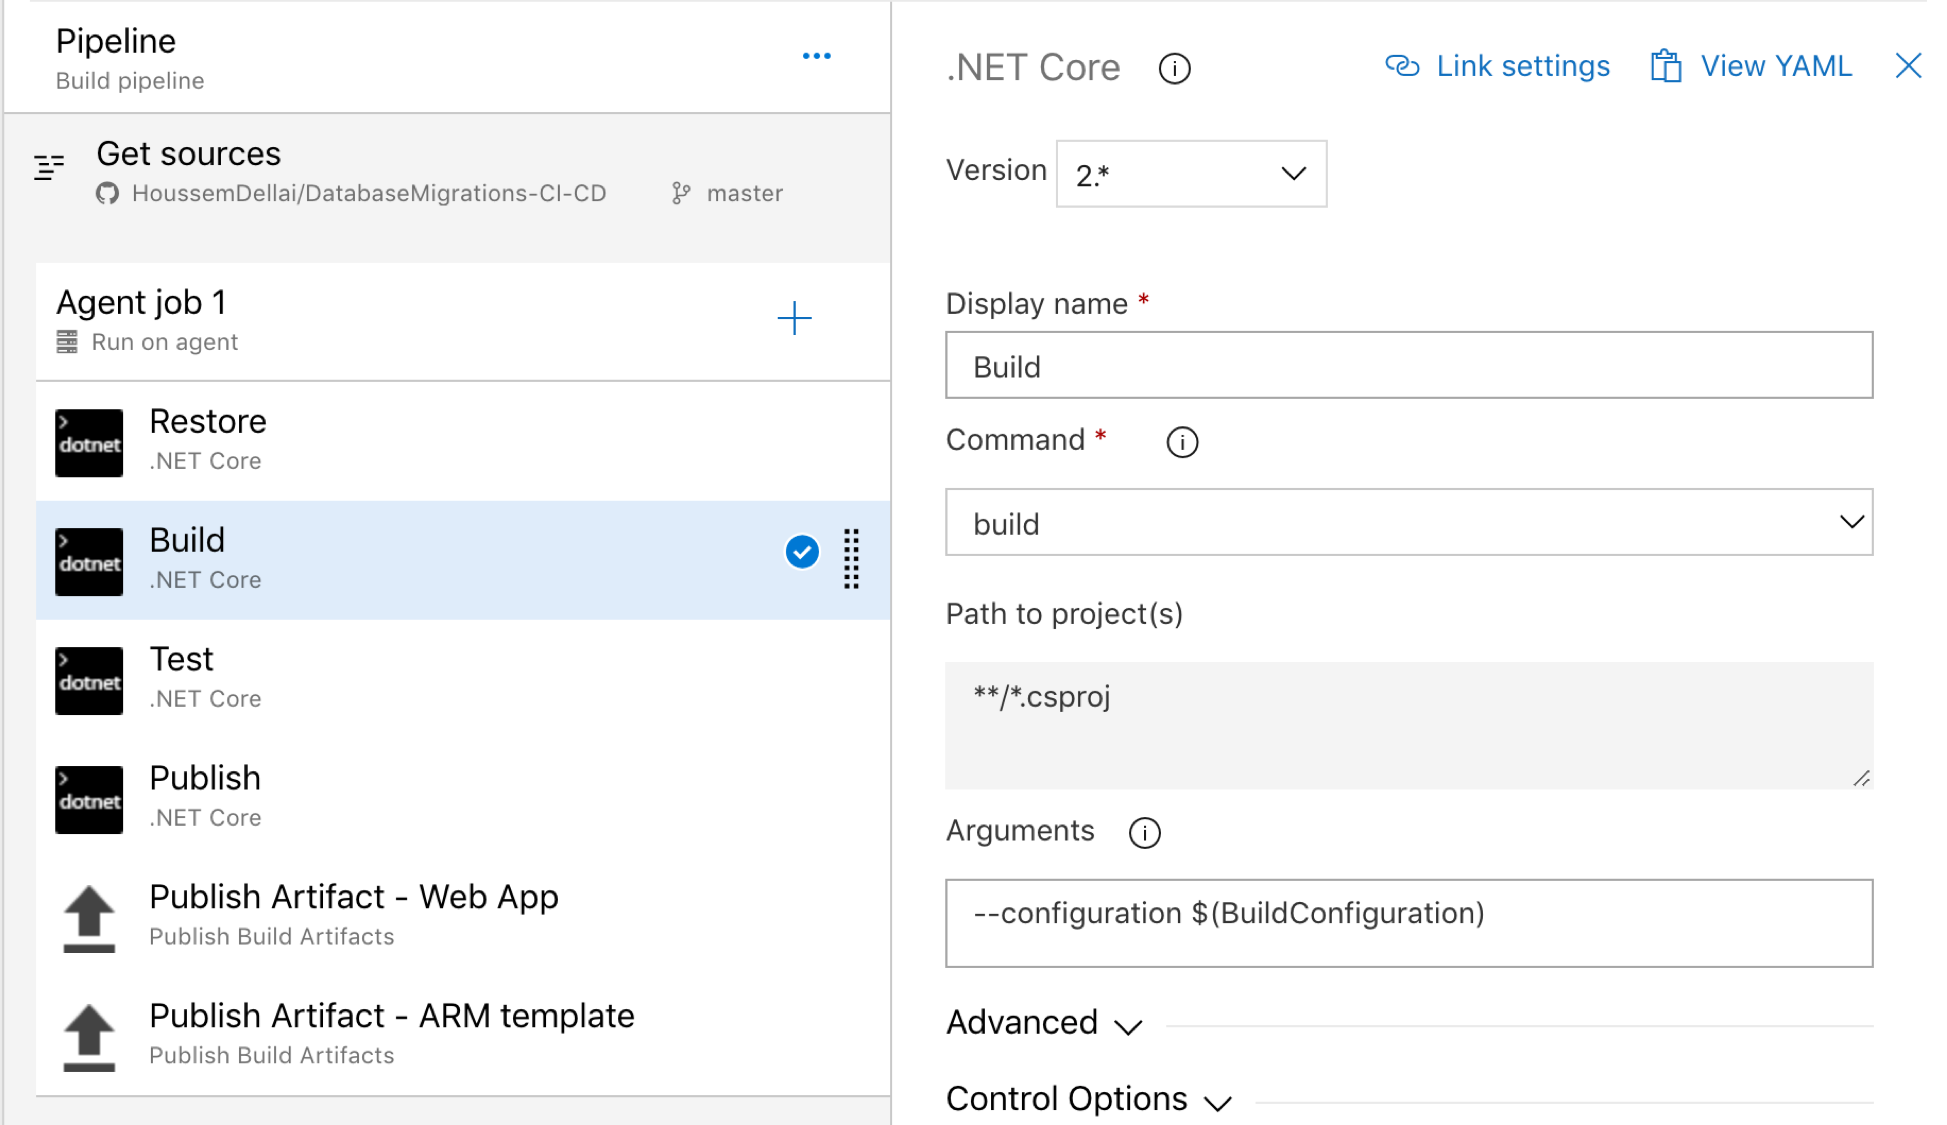
\includegraphics[width=12cm,height=7cm]{./IMAGENES/analisis2}
			\end{center}
			Houssem Dellai(2018).DevOps para la base de datos:.[Figura].Recuperado de 
https://medium.com/faun/devops-for-database-4e442abfd939
		\end{figure}

	Y nuestro canal de lanzamiento / CD tendrá el siguiente aspecto, donde solo publicaremos el paquete generado en Azure App Service. Durante esa operación, las migraciones se ejecutarán al reiniciar la aplicación. También puede observar la primera tarea que implementará la plantilla ARM en Azure.

	\begin{figure}[H]
			\begin{center}
					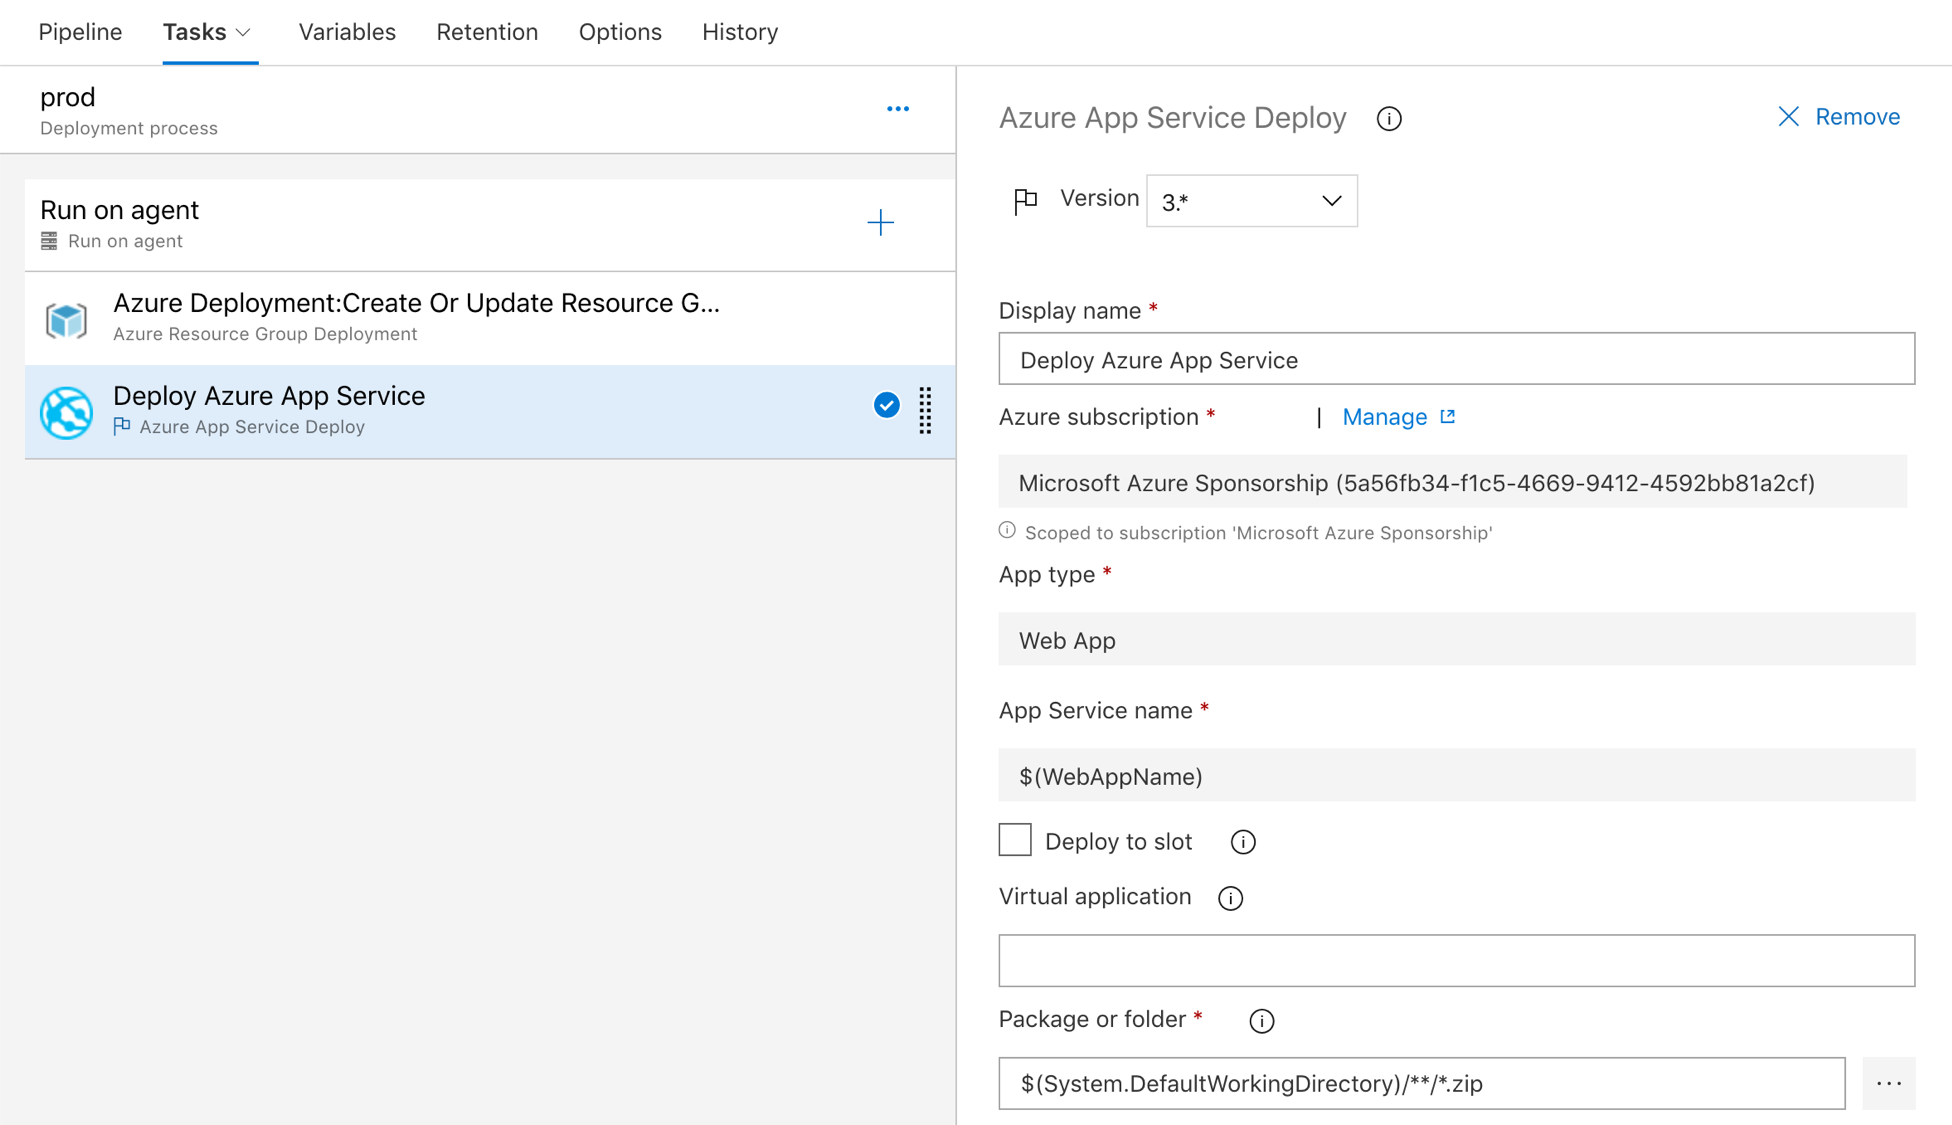
\includegraphics[width=12cm,height=7cm]{./IMAGENES/analisis3}
			\end{center}
			Houssem Dellai(2018).DevOps para la base de datos:.[Figura].Recuperado de 
https://medium.com/faun/devops-for-database-4e442abfd939
		\end{figure}

Sin embargo, este enfoque es adecuado solo para proyectos pequeños donde no hay DBA, el esquema de la base de datos es bastante simple y sobre todo: ¡le damos control total y confianza al ORM para administrar la base de datos!.

\subsection{Ejecutar el script de migración generado por el ORM}
Bueno, podemos recuperar algo de control. Dejaremos que ORM genere los scripts SQL. Pero luego iremos a leerlo, editarlo, validarlo e implementarlo.
Para eso, necesitamos ejecutar una línea de comando para interceptar los scripts SQL generados: dotnet ef migrations script -o outputfile.sql
		\begin{figure}[H]
			\begin{center}
					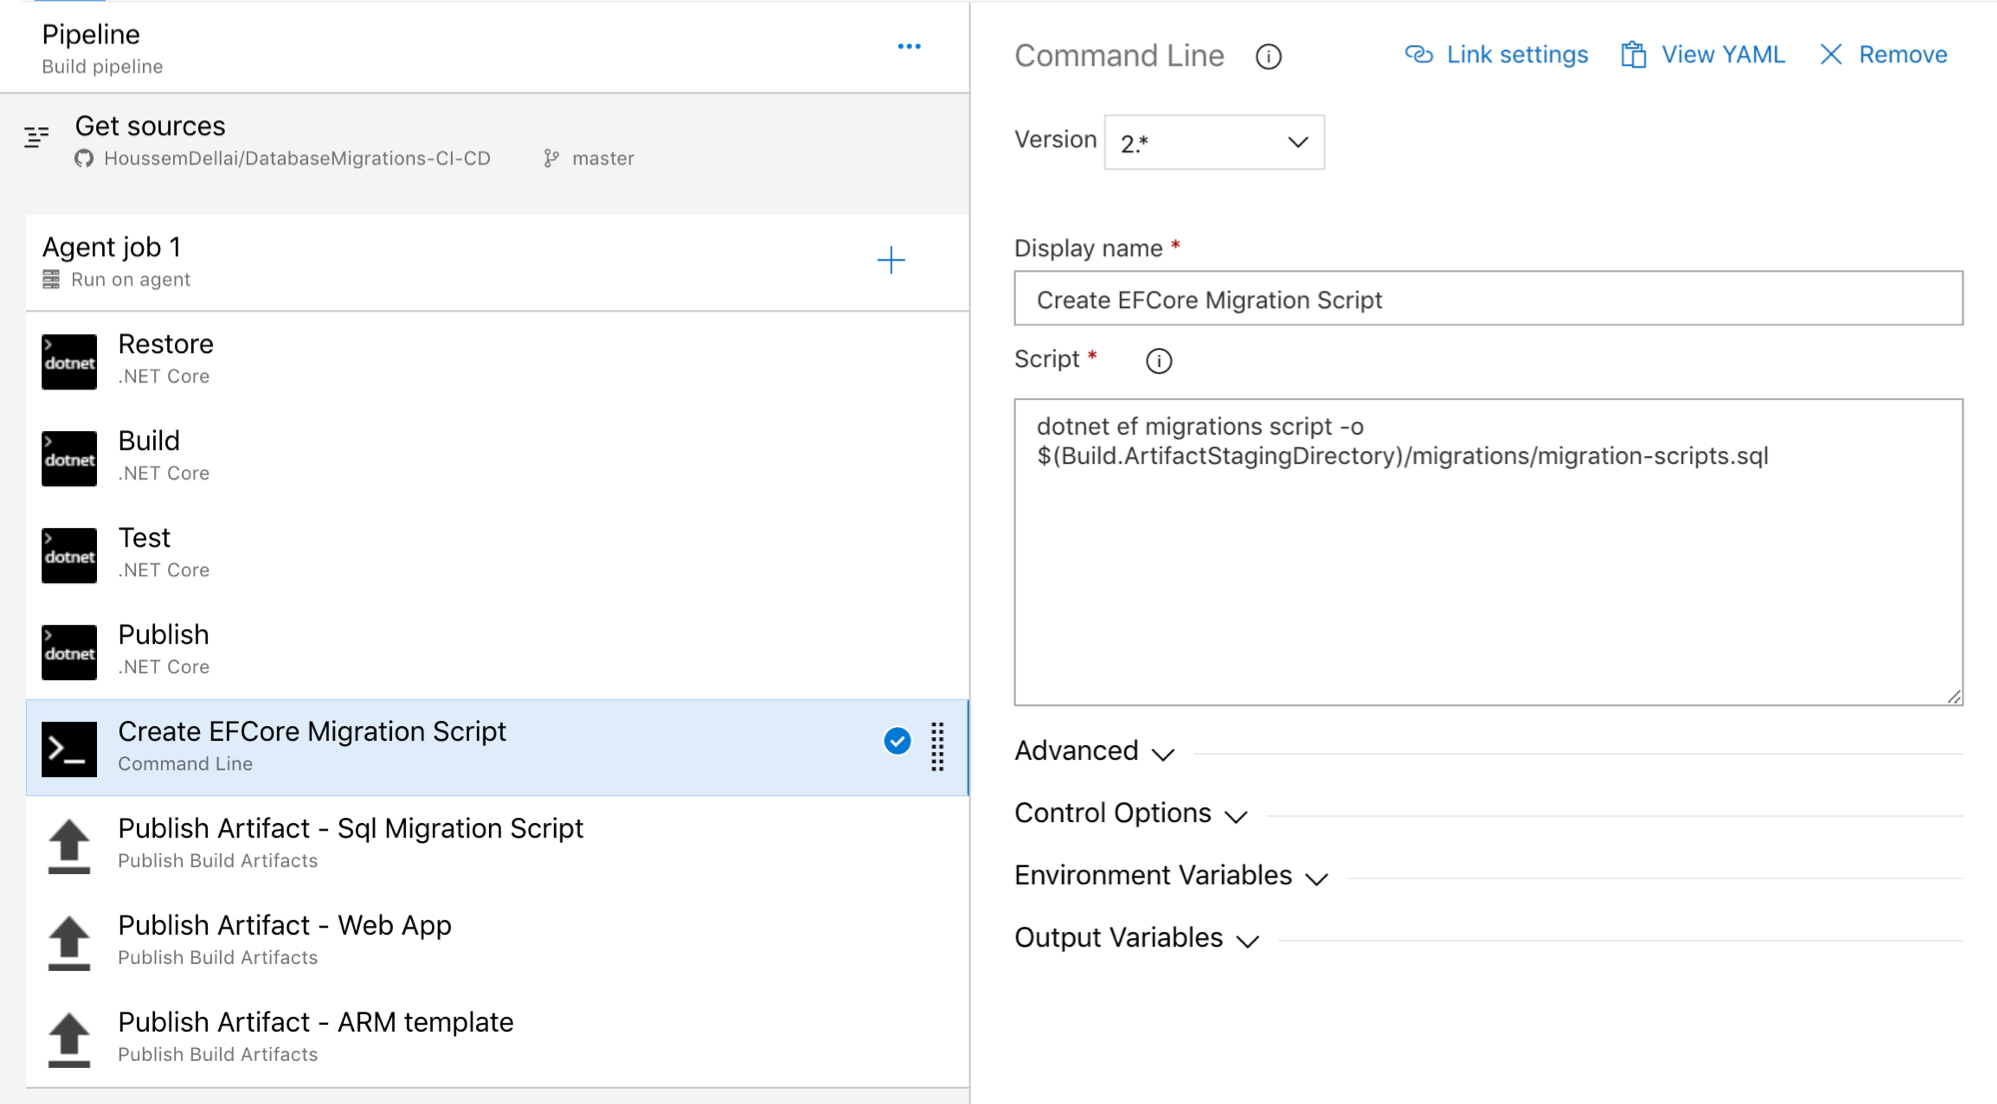
\includegraphics[width=12cm,height=7cm]{./IMAGENES/analisis4}
			\end{center}
			Houssem Dellai(2018).DevOps para la base de datos:.[Figura].Recuperado de 
https://medium.com/faun/devops-for-database-4e442abfd939
		\end{figure}
	Obtendremos el script generado y lo subiremos a la carpeta drop o artifact para que podamos acceder a él durante la canalización del CD. Eso se hace mediante la tarea Publicar artefacto. Cuando finalice la compilación, podemos ver y editar los scripts generados.
Ahora, desde la canalización de CD, implementaremos el script en la base de datos directamente. Para eso, necesitamos conectarnos a la base de datos alojada en Azure. Esa es la función de la tarea Azure SQL Publish. Utilizará la herramienta cll sqlcmd debajo del capó.

	\begin{figure}[H]
			\begin{center}
					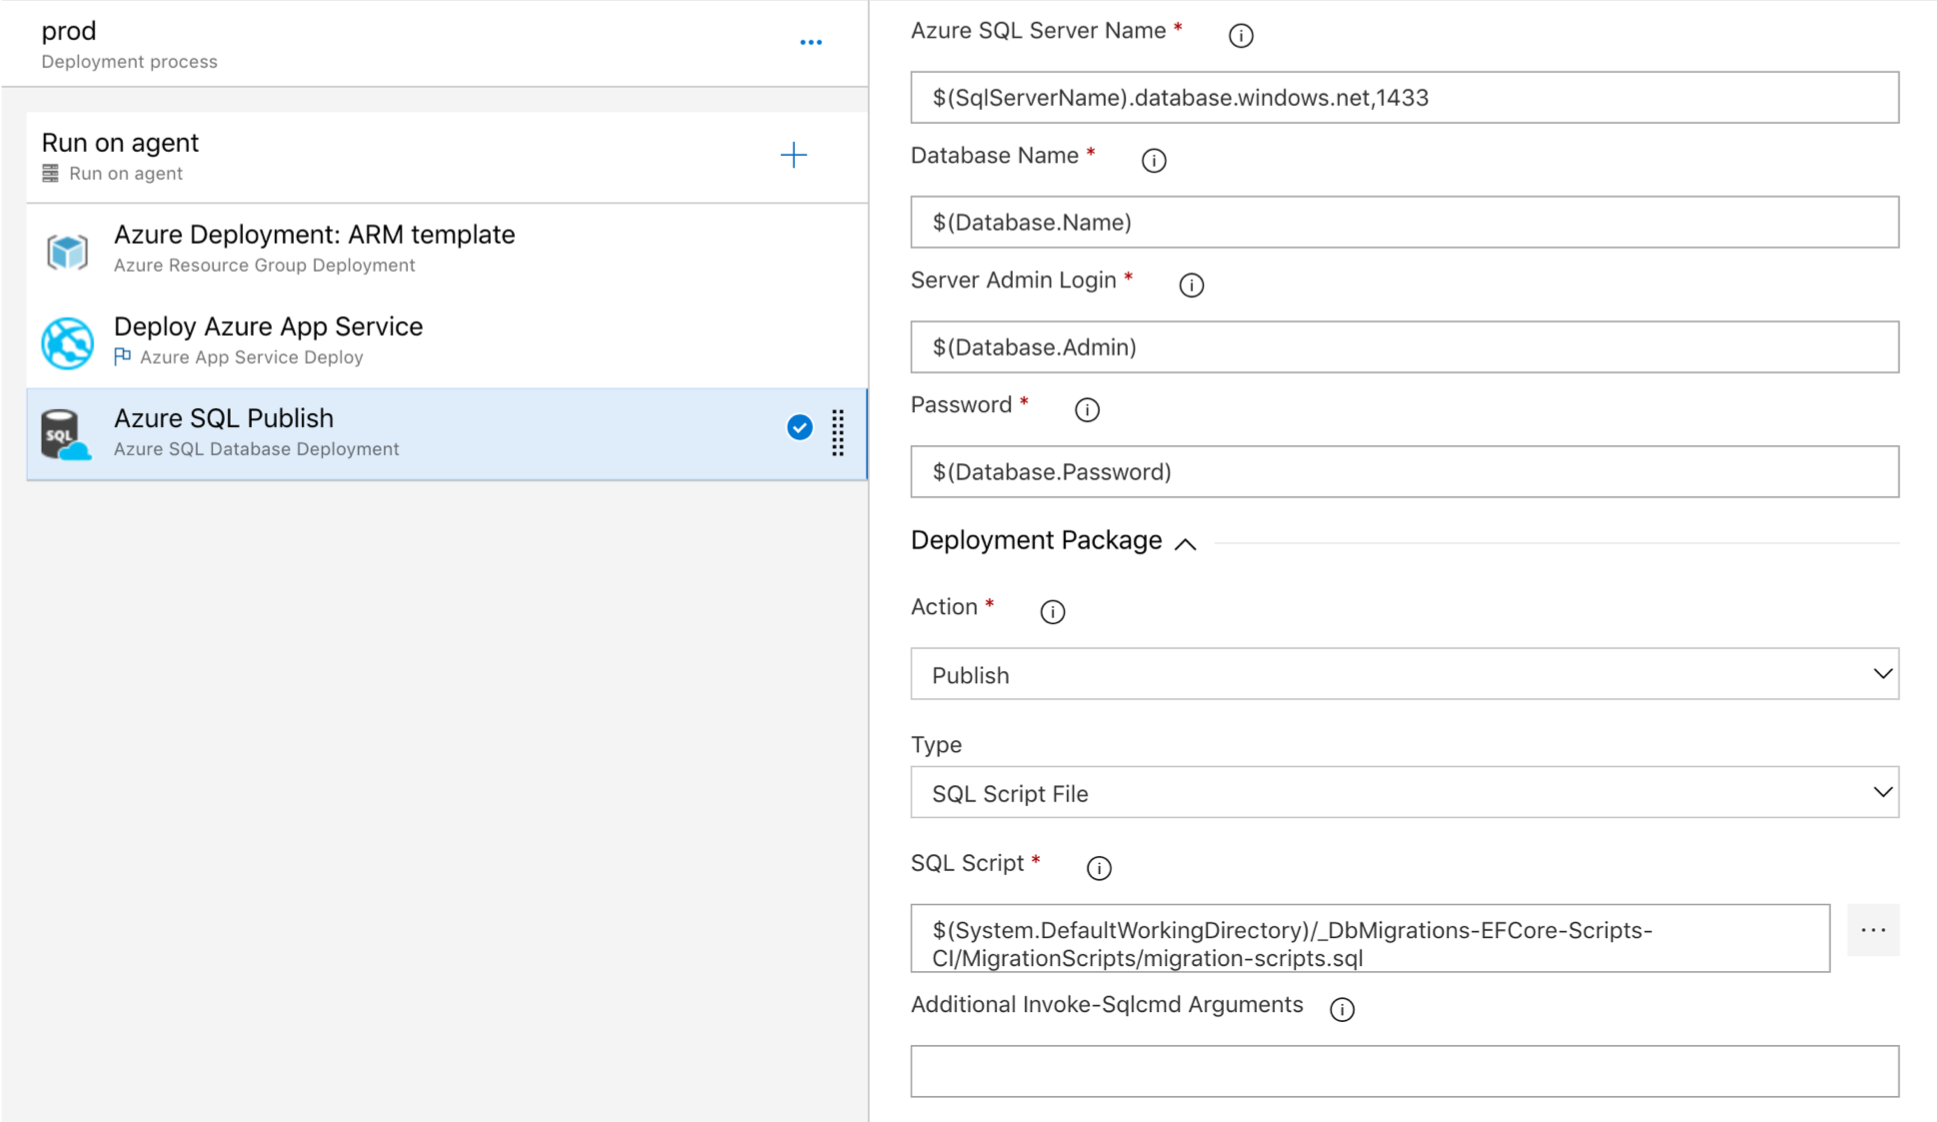
\includegraphics[width=12cm,height=7cm]{./IMAGENES/analisis5}
			\end{center}
			Houssem Dellai(2018).DevOps para la base de datos:.[Figura].Recuperado de 
https://medium.com/faun/devops-for-database-4e442abfd939
		\end{figure}
\subsection {Usando el proyecto de base de datos}
Aún así, para proyectos más grandes, los DBA crean tipos de proyectos separados para administrar la base de datos. Estos proyectos contienen, generan y validan consultas SQL. Estamos hablando del proyecto de base de datos que se podría abrir desde Visual Studio, pero también desde SQL Server Management Studio (SSMS), que es la herramienta favorita para los DBA. Con este enfoque, DBA tendrá control total sobre la generación de los scripts SQL.

\begin{figure}[H]
			\begin{center}
					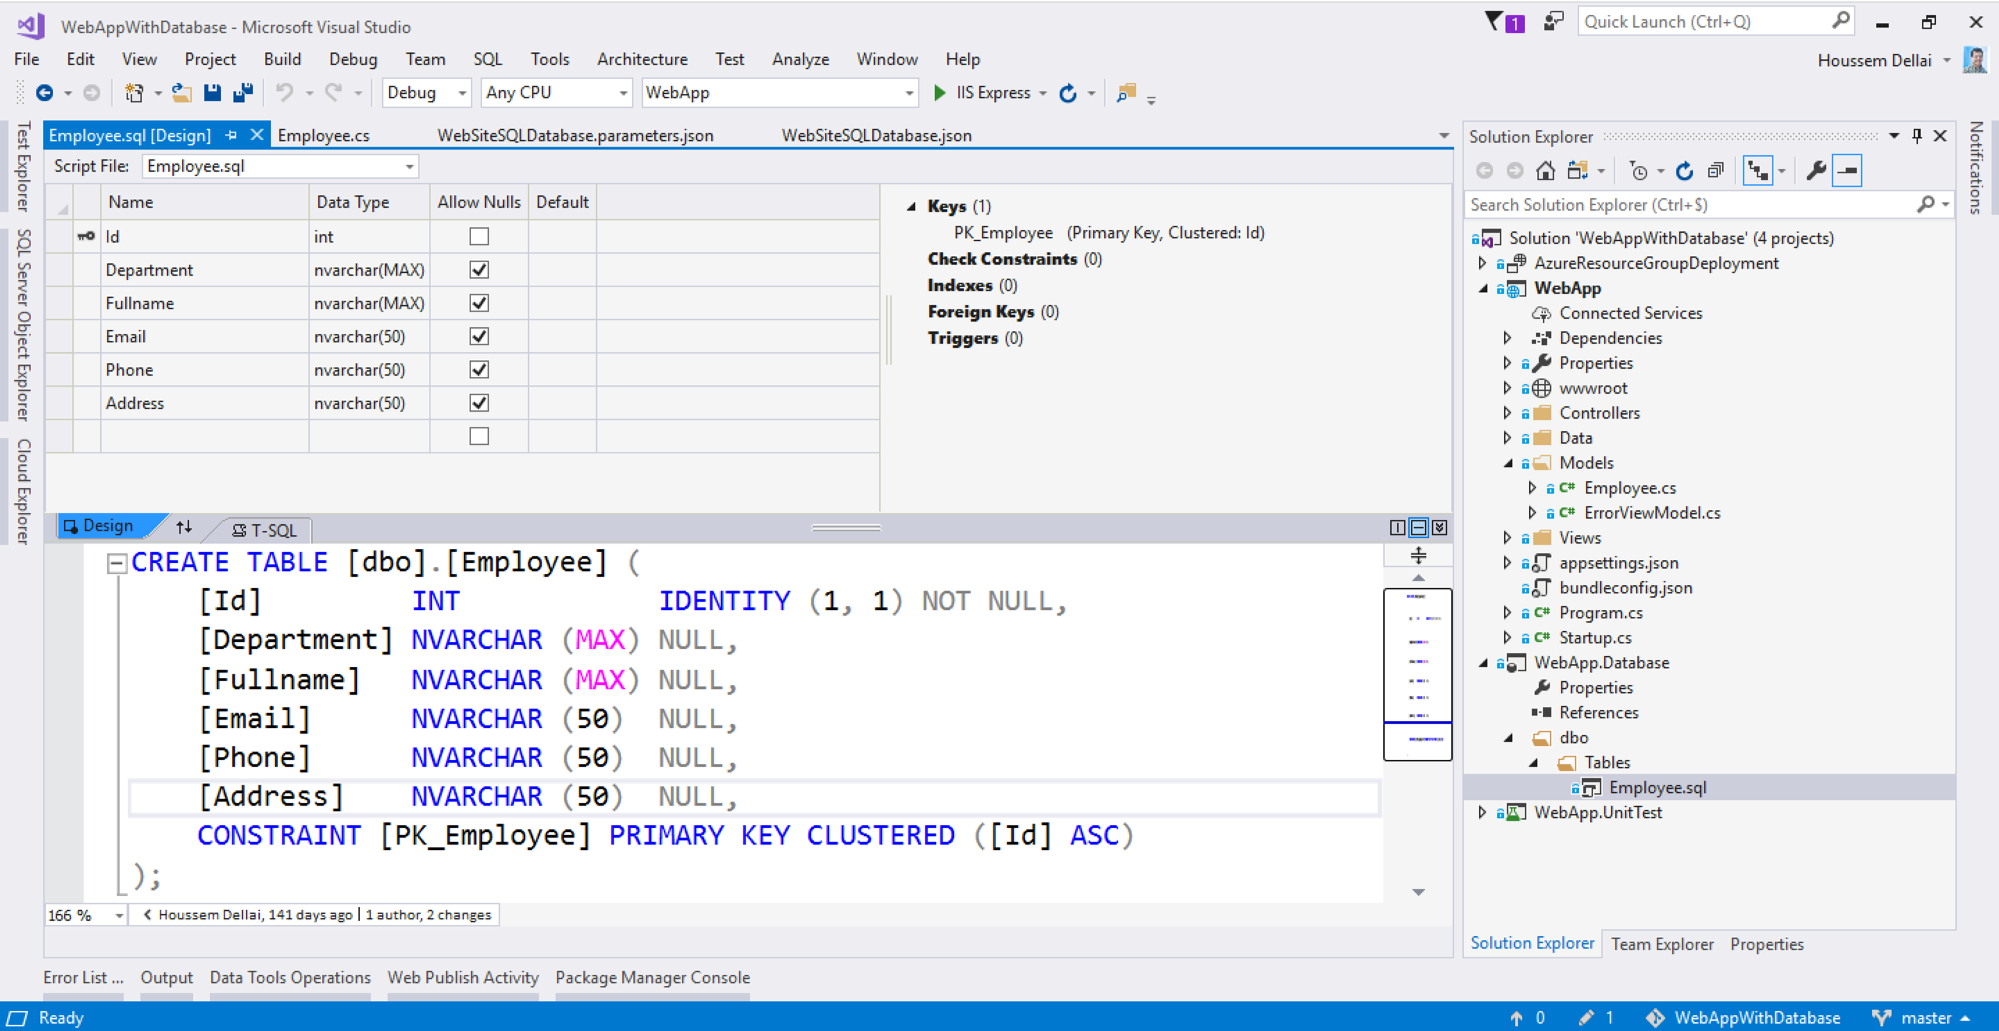
\includegraphics[width=12cm,height=7cm]{./IMAGENES/analisis6}
			\end{center}
			Houssem Dellai(2018).DevOps para la base de datos:.[Figura].Recuperado de 
https://medium.com/faun/devops-for-database-4e442abfd939
		\end{figure}

Ahora, la generación de los scripts SQL será realizada manualmente por DBA, ya no será administrada por ORM. Estamos de acuerdo con eso, ya que creemos que los DBA son más inteligentes que ORM, especialmente para prevenir y resolver conflictos.

Solo necesitamos construir el proyecto para generar un archivo DacPac que contenga el nuevo esquema creado usando los scripts provistos. Tenga en cuenta que en la siguiente imagen podríamos construir el proyecto de la base de datos en un agente / fase separada, ya que no depende de los proyectos de la aplicación. Eso es útil si queremos ejecutarlos en paralelo.

\begin{figure}[H]
			\begin{center}
					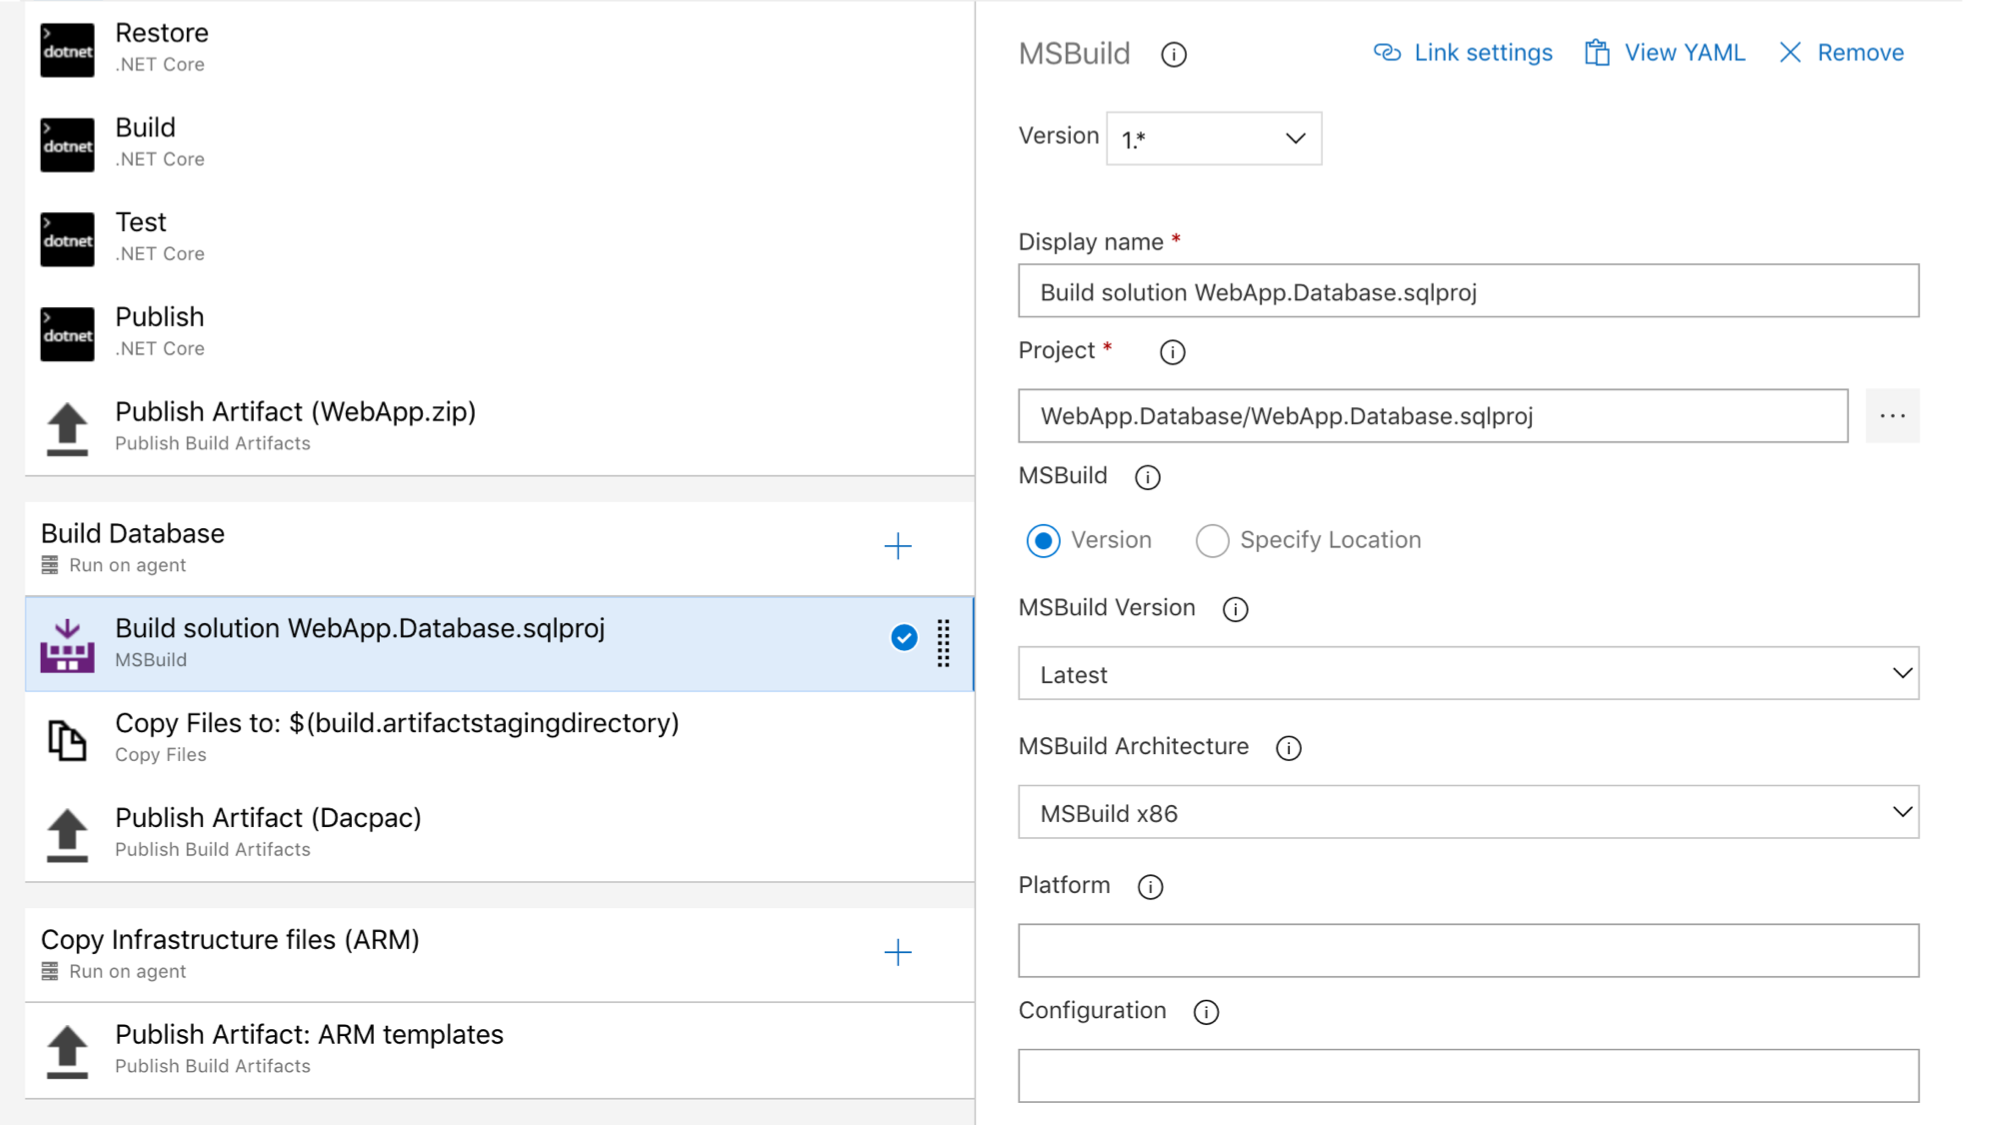
\includegraphics[width=12cm,height=7cm]{./IMAGENES/analisis7}
			\end{center}
			Houssem Dellai(2018).DevOps para la base de datos:.[Figura].Recuperado de 
https://medium.com/faun/devops-for-database-4e442abfd939
		\end{figure}

Para la canalización de CD, implementaremos el DacPac en la base de datos. Usaremos la misma tarea que antes: implementación de la base de datos SQL Azure, pero en lugar de publicar un script SQL, le diremos que publique el DacPac.

\begin{figure}[H]
			\begin{center}
					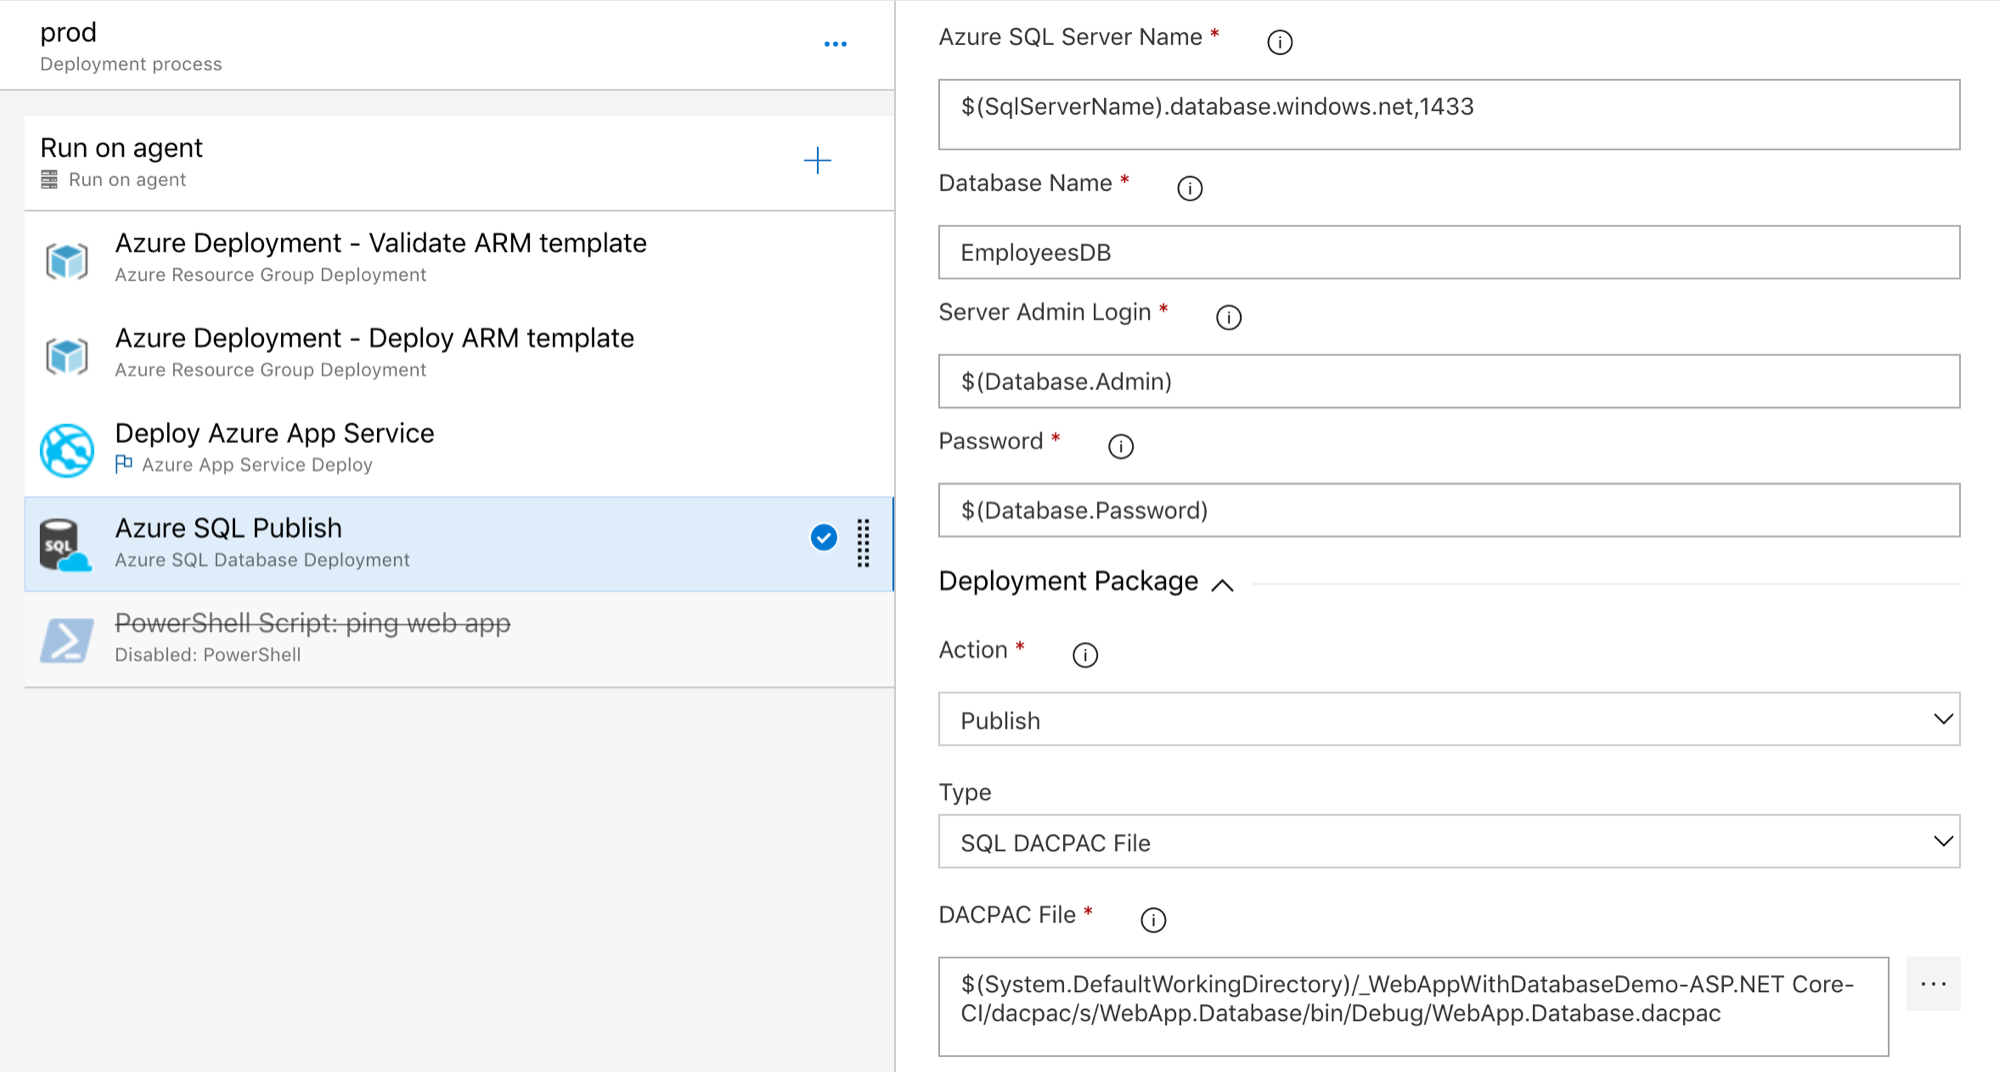
\includegraphics[width=12cm,height=7cm]{./IMAGENES/analisis8}
			\end{center}
			Houssem Dellai(2018).DevOps para la base de datos:.[Figura].Recuperado de 
https://medium.com/faun/devops-for-database-4e442abfd939
		\end{figure}



\section{Conclusion}
\begin{itemize}
\item Conclusion : \\


Las implementaciones de bases de datos pueden ser más rápidas, fáciles y libre de errores al extender las prácticas de DevOps a las bases de datos. Ha demostrado cómo el desarrollo y los equipos de operaciones pueden organizar los procesos de la base de datos para proteger mejor los datos. También ha destacado la importancia de la entrega continua de bases de datos para alentar la organización y los equipos de desarrollo y operaciones para trabajar juntos para construir y entregar un excelente software.

\end{itemize}

	
	\newpage
	
	\bibliographystyle{apalike} 	
	\bibliography{BIBLIOGRAFIA}	 
\citep{referencia01}  
\citep{referencia02}  
\citep{referencia03}  
\citep{referencia04}  
\citep{referencia05}  
\citep{referencia06}  
\citep{referencia07}  
\citep{referencia08} 
\citep{referencia09}

\end{document}

